\documentclass[letterpaper]{article}
\usepackage[submission]{aaai2027}
\usepackage{times,helvet,courier}
\usepackage[hyphens]{url}
\usepackage{graphicx}
\usepackage{natbib}
\usepackage{caption}
\usepackage{booktabs,amsmath,amssymb,array,xspace}
\frenchspacing
\urlstyle{rm}
\def\UrlFont{\rm}
\pdfinfo{/TemplateVersion (2027.1)}
\setcounter{secnumdepth}{2}
\newcommand{\method}{TRACE\xspace}
\newcommand{\sg}{\operatorname{sg}}
\newcommand{\pending}{\textit{pending}}
\newcommand{\mainref}[1]{\ref{#1}}

\title{TRACE: Context-Probed Region Allocation for Test-Time Adaptation\\in Open-Vocabulary Semantic Segmentation}
\author{Anonymous Authors}
\affiliations{}
\begin{document}
\raggedbottom
\maketitle

\begin{abstract}
Test-time adaptation for open-vocabulary semantic segmentation learns from the model's own dense predictions, making the choice of self-supervision central to the update. Initial confidence alone does not reveal whether a local prediction remains supported when its surroundings change. We propose TRACE, which uses this additional response to allocate adaptation across predicted regions. A single context probe preserves each candidate's pixels, changes its surroundings, and measures support for the original text query at the same locations. The resulting scores weight regional entropy; region averaging and within-image normalization separate relative priority from explicit area and cross-image support multipliers. This design retains contextual information for segmentation while using its perturbation to guide adaptation. Across eight full-split benchmark protocols, TRACE improves over initial-confidence weighting, including gains of 3.13 mIoU on VOC21, 3.31 on COCO Object, and 9.57 on COCO-CD. These results show that context-probed support can provide useful update-allocation information beyond confidence, using one diagnostic input per candidate.
\end{abstract}

\section{Introduction}
Open-vocabulary semantic segmentation (OVSS) extends dense recognition to categories specified by text, using the transferable representations of vision--language models~\cite{radford2021clip,hajimiri2025naclip}. Test-time adaptation (TTA) further adjusts these representations using unlabeled inputs. Its supervision, however, comes from the model being adapted: entropy minimization strengthens current predictions, including predictions that may be incorrect~\cite{wang2021tent,noori2025mlmp}. The central question is therefore not just how to sharpen a segmentation, but which predicted regions should have greater influence on that update.

Initial confidence leaves part of this decision unresolved because a spatial prediction is computed from contextualized features. Although its token lies inside a candidate region, its representation can incorporate information from elsewhere in the image. Patch alignment, local self-distillation, and modified token interactions improve the transfer from image--text learning to dense prediction~\cite{mukhoti2023pacl,wu2024clipself,shao2024cliptrase}; object--context and region--language studies also examine the influence of neighboring semantics~\cite{kim2025cass,li2025densevlm}. For adaptation, a further distinction matters: a strong response in the observed image does not tell us whether the same region remains supported after its surrounding content changes.

Our starting point is to use a change in context as a diagnostic signal rather than remove context from segmentation. Surrounding information can aid recognition~\cite{xiao2021backgrounds}, so TRACE preserves the original image for adaptation and final inference. For diagnosis, it keeps a candidate's pixels unchanged, modifies only the surroundings, and measures the original category response at the same locations. Figure~\ref{fig:teaser} shows that initially confident candidates can have different support under this probe. This additional observation offers a way to distinguish their relative contributions to self-supervision without requiring labels or a separate region-proposal model.

\begin{figure}[t]
\centering
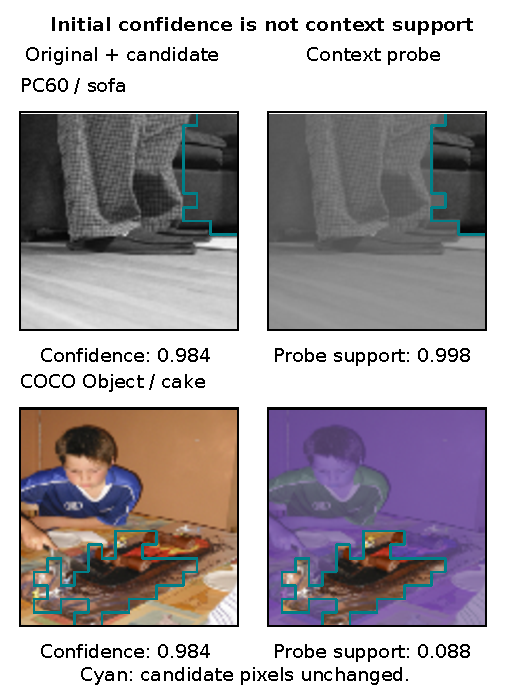
\includegraphics[width=\columnwidth]{figure/tuned/image_full_teaser.pdf}
\caption{Confidence and context-probed support capture different aspects of a prediction. Each probe preserves the candidate pixels and changes only their surroundings; scores are read at the original candidate locations. The displayed examples illustrate the distinction. Case selection is detailed in Appendix~\ref{app:figures}.}
\label{fig:teaser}
\end{figure}

TRACE translates context-probed support into \emph{regional allocation}: the relative influence of predicted regions on the adaptation objective. Connected components of the initial prediction provide local candidates, and confidence top-$K$ bounds the number of probes. Each candidate's measured support then weights its regional average entropy. Two normalization choices make this allocation explicit: averaging entropy within a region avoids a direct area multiplier, while normalizing weights within each source image prevents its total support from determining its share of the loss. The method thus distinguishes where to allocate supervision from how much image area a region occupies.

Matched comparisons test whether this extra observation improves adaptation when candidates and optimization settings are held fixed. TRACE improves over initial-confidence weighting across eight full-split protocols, including VOC21 (+3.13 mIoU), COCO Object (+3.31), and COCO-CD (+9.57). The gains vary across datasets, reaching +0.11 on COCO-Stuff: the value of the probe depends on its effect on adaptation, rather than being assumed from confidence or support alone. Single- and dual-probe comparisons examine how much diagnostic information is needed, while measured execution costs quantify the price of acquiring it.

Our contributions are:
\begin{itemize}
\item We introduce context-probed regional allocation for OVSS adaptation: support after a candidate-preserving context change guides how strongly each region contributes to self-supervision.
\item We formulate an image-balanced regional entropy objective that separates support-based priority from explicit region-area and cross-image support multipliers.
\item We establish the value of the additional response through matched allocation controls, and characterize the accuracy--computation tradeoff of a single-probe design.
\end{itemize}

\section{Related Work}
\paragraph{Open-vocabulary dense prediction.}
OVSS transfers vision--language representations through dense matching, mask classification, or segmentation-oriented adaptation~\cite{ghiasi2022openseg,liang2023ovseg,cho2024catseg}. PACL aligns local patches with language, while CLIPSelf distills local visual features~\cite{mukhoti2023pacl,wu2024clipself}. NACLIP and CLIPtrase modify or analyze spatial-token interactions for training-free segmentation~\cite{hajimiri2025naclip,shao2024cliptrase}. TRACE addresses the subsequent allocation of test-time self-supervision, using the dense predictor as its inference interface.

\paragraph{Test-time adaptation.}
TENT optimizes entropy through normalization-affine parameters~\cite{wang2021tent}. CoTTA, EATA, and SAR introduce consistency, selection, or optimization controls~\cite{wang2022cotta,niu2022eata,niu2023sar}. TPT and WATT adapt vision--language models through prompts or template-associated weights~\cite{shu2022tpt,osowiechi2024watt}; Seg-TTO and SemLA address segmentation-specific adaptation~\cite{desilva2025segtto,qorbani2025semla}. MLMP combines visual levels and prompt-specific entropy with a global image-level term~\cite{noori2025mlmp}. TRACE retains dense prompt-specific entropy but assigns its influence through candidate-context responses and within-image regional normalization.

\paragraph{Context and model probing.}
Background-dependence studies distinguish recognition from the evidence sustaining it~\cite{xiao2021backgrounds}. CASS models object--context relations in OVSS, while DenseVLM examines biases in region--language alignment~\cite{kim2025cass,li2025densevlm}. Perturbation-based explanations inspect model behavior under controlled input changes~\cite{fong2019extremal,zhang2020conta}. TRACE uses a fixed, candidate-preserving perturbation to obtain relative update weights; it does not train an explanation model or assume calibrated probabilities of correctness.

\section{Method}
\label{sec:method}
An episode starts from reset model parameters $\theta_0$ and unlabeled source images $X_j$. TRACE selects connected predicted regions, measures their support under a candidate-preserving context change, and uses fixed regional weights to adapt the visual encoder. Figure~\ref{fig:pipeline} summarizes these three steps. Diagnostics never use image annotations.

\begin{figure*}[!t]
\centering
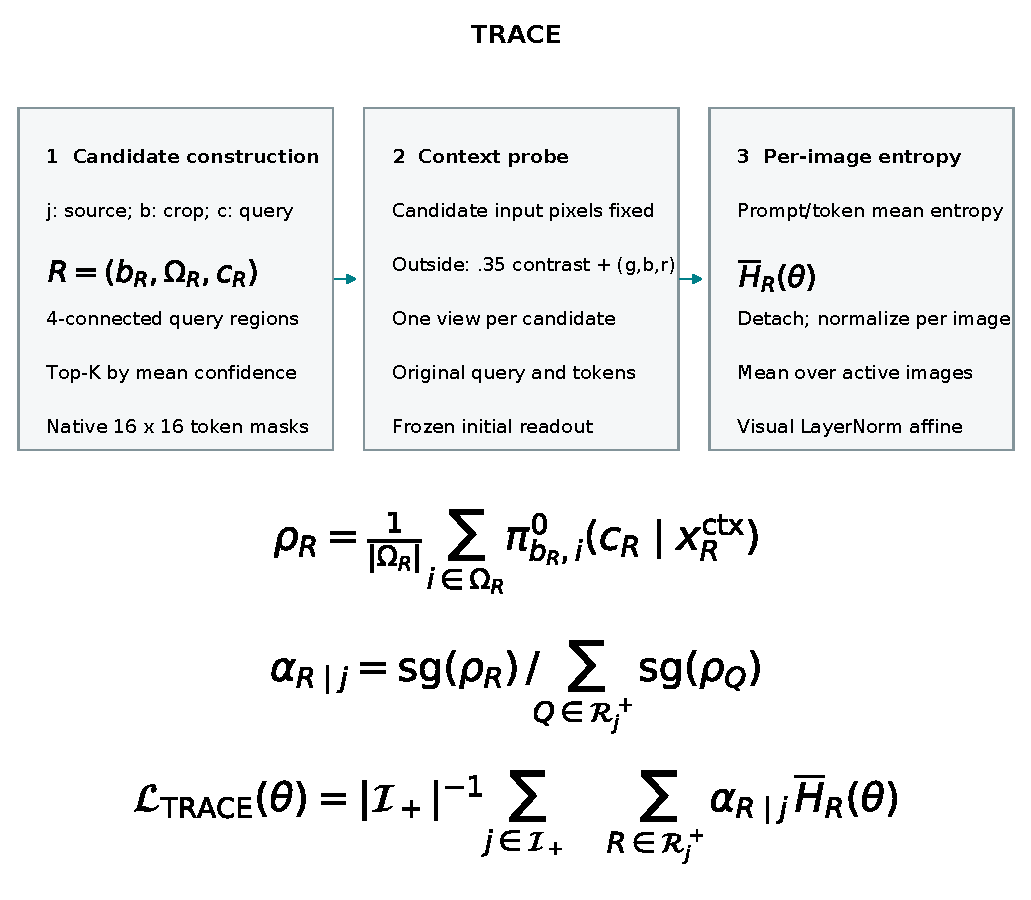
\includegraphics[width=\textwidth]{figure/tuned/image_full_pipeline.pdf}
\caption{TRACE with one context probe per candidate. Initial token predictions define connected regions and source-image top-$K$ selection. Each candidate keeps its pixels while its surroundings undergo the fixed transform. The reset encoder measures the candidate query at its original token locations. Detached scores are normalized within source images and weight regional prompt entropy on unmodified inputs. Only visual LayerNorm affine parameters update; the inference readout reconstructs the final segmentation.}
\label{fig:pipeline}
\end{figure*}

\subsection{Candidate Region Construction}
Regions let adaptation distinguish spatially separate predictions without diagnosing every token independently. We use connected components of the initial segmentation so that candidates follow the model's own local predictions and require neither instance annotations nor a separate proposal network. A candidate is a connected prediction component; it need not correspond to a complete physical object.

Each source image is preprocessed into normalized input crops $x_b$, with source index $j(b)$. A $224\times224$ crop contains $16\times16$ spatial tokens for ViT-L/14; a ViT patch is distinct from an input crop. Let $\mathcal C$ be the text-query vocabulary, including any extensions. It need not equal the final evaluation-category set $\mathcal Y$. The reset diagnostic branch defines
\begin{equation}
\pi^0_{b,i}(c\mid x_b)=\operatorname{softmax}_{c\in\mathcal C}
z^{\mathrm{eval}}_{\theta_0}(x_b)_{i,c}.
\label{eq:reference}
\end{equation}
This branch uses normalized mean prompt embeddings and entropy-weighted visual-layer aggregation. Gradient-bearing optimization uses separate prompt distributions; Appendix~\ref{app:readout} specifies both readouts.

For each crop, we take the query argmax and extract four-neighbor connected components within its valid token mask. A candidate $R=(b_R,\Omega_R,c_R)$ records the crop, token locations, and predicted query. Its initial confidence is $\kappa_R=|\Omega_R|^{-1}\sum_{i\in\Omega_R}\pi^0_{b_R,i}(c_R\mid x_{b_R})$. Proposals from all crops of the same source image compete for its top-$K$ positions by descending $\kappa_R$; deterministic tie rules appear in Appendix~\ref{app:protocol}. The selected set for image $j$ is $\mathcal R_j$.

Confidence bounds the diagnostic workload and identifies predictions likely to be used for self-supervision; it does not certify reliability. The next module assigns weights independently of the initial rank. Components are not stitched across crops or merged across query extensions, even when extensions map to the same final category. Candidate geometry and query identities remain fixed within the episode.

\subsection{Candidate-Preserving Context Probe}
The probe tests a prediction while retaining the local content that produced it. Changing the candidate itself would entangle loss of target content with sensitivity to context. We instead preserve candidate pixels, transform only their surroundings, and read the original query at the original locations. The same construction applies to all categories.

Let $u=\operatorname{Denorm}(x_{b_R})$ be the crop in RGB pixel space, and $M_R$ its token mask upsampled by nearest-neighbor interpolation to the crop dimensions. For the crop's per-channel spatial mean $\mu$, define
\begin{equation}
A(u)=\operatorname{clip}_{[0,255]}
\left(\operatorname{Shift}\bigl(\mu+0.35(u-\mu)\bigr)\right),
\end{equation}
where $\operatorname{Shift}(r,g,b)=(g,b,r)$. The diagnostic input is
\begin{equation}
x_R^{\mathrm{ctx}}=\operatorname{Norm}
\left(M_R\odot u+(1-M_R)\odot A(u)\right).
\label{eq:context-view}
\end{equation}
Only the mask complement is replaced. The response uses the original query and token locations:
\begin{equation}
\rho_R=\frac{1}{|\Omega_R|}\sum_{i\in\Omega_R}
\pi^0_{b_R,i}(c_R\mid x_R^{\mathrm{ctx}}).
\label{eq:support}
\end{equation}
This is a mean of probabilities, not logits. No new region is extracted from the transformed prediction. The score measures support under this context change, not invariance to every possible context. We call this probe mode $C$ in the comparisons below.

Each region receives its own transformed input, but regions do not require serial model calls. We index views by candidate, stack them into bounded batches, and map their logits back to the corresponding candidate before averaging over $\Omega_R$. Diagnostic inputs therefore number one per candidate, while encoder calls depend on view batch size. The resulting scores are detached and fixed during the episode.

\subsection{Image-Balanced Regional Adaptation}
The objective separates three decisions: which regions receive priority, how their pixels are aggregated, and how images share the loss. Summing token losses would give a larger region more influence simply because it contains more tokens. Likewise, normalizing all regional scores across an episode would give images with greater total support a larger coefficient share. TRACE averages entropy within regions, distributes a normalized budget among each image's candidates, and then averages image objectives.

Let $p^a_{\theta,b,i}$ be the current query distribution for prompt $a\in\{1,\ldots,J\}$ on an unmodified crop, and $H(p)=-\sum_{c\in\mathcal C}p(c)\log p(c)$. Each candidate has mean prompt/token entropy
\begin{equation}
\overline H_R(\theta)=\frac{1}{J|\Omega_R|}
\sum_{a=1}^{J}\sum_{i\in\Omega_R}H\bigl(p^a_{\theta,b_R,i}\bigr).
\end{equation}
Define active regions $\mathcal R_j^+=\{R\in\mathcal R_j:\rho_R>\epsilon\}$, with the fixed numerical threshold $\epsilon=10^{-8}$, and active images $\mathcal I_+=\{j:\mathcal R_j^+\neq\varnothing\}$. We optimize
\begin{align}
\alpha_{R\mid j}&=\frac{\sg(\rho_R)}
{\sum_{Q\in\mathcal R_j^+}\sg(\rho_Q)},\\
\mathcal L_{\mathrm{TRACE}}(\theta)&=\frac{1}{|\mathcal I_+|}\sum_{j\in\mathcal I_+}
\sum_{R\in\mathcal R_j^+}\alpha_{R\mid j}\overline H_R(\theta).
\label{eq:loss}
\end{align}
Here $\sg$ denotes stop-gradient. Images without active candidates contribute no term; if no image is active, adaptation is skipped. The candidate query selects the diagnostic response but is not a cross-entropy pseudo-label for this entropy objective.

Each active image has total coefficient mass $1/|\mathcal I_+|$. Within it, $\alpha_{R\mid j}$ gives relative regional priority without an explicit area multiplier. This is a loss-budget property, not equality of gradient norms or invariance to batch composition. Common positive scaling of an image's active scores cancels; a singleton candidate's positive score also cancels. Support thus controls relative allocation, not the absolute learning rate or number of updates (Appendix~\ref{app:theory}).

Only visual LayerNorm affine parameters update using Adam; the text encoder and other visual parameters remain frozen. Model and optimizer reset before each episode. Final inference uses unmodified inputs, reconstructs pixel query scores, and takes the maximum over extensions of each evaluation category before category argmax. Appendix~\ref{app:protocol} gives this coordinate and vocabulary mapping.

\section{Experiments}
\subsection{Experimental Setup}
The experiments address one central question: does a region's response to changed context provide useful adaptation information beyond its initial confidence? We first isolate this choice with matched regional-weighting controls, then compare segmentation performance with published and local references. Probe alternatives and measured execution costs examine the information--computation tradeoff.

\paragraph{Datasets and implementation.}
Evaluation covers VOC20/VOC21 (1,449 images each), PC59/PC60 (5,105 each), COCO Object (5,000), COCO-Stuff (5,000), COCO-CD (500), and Waterbirds-Seg (5,322). The VOC and PC pairs respectively share images with different category sets. We report mIoU from per-class intersections and unions pooled over each complete split. All local controls use the same NACLIP ViT-L/14 checkpoint, last 18 visual outputs, and seven prompts. Images and labels are resized to $224\times224$ with nearest-neighbor label interpolation, giving one input crop per image. Results therefore refer to this resized evaluation setting. Exact configurations and readouts are provided in Appendix~\ref{app:protocol}.

\paragraph{Comparison protocol.}
Uniform, Confidence, and TRACE hold candidates, input order, readouts, and optimization settings fixed; only the regional weights and requested diagnostic views differ. No Adapt evaluates the reset model without updates. Each adapting method resets both model and optimizer before an episode. The common context probe is fixed before per-dataset parameter selection. Batch size, learning rate, steps, and $K$ are selected on fixed 256-image training-source panels, with at most 80 configurations per dataset; Uniform and Confidence use the selected TRACE configuration without separate tuning. All eight configurations are fixed before full evaluation, which uses seed 0. The datasets have historical development exposure; additionally, the 256 Waterbirds calibration images belong to its original 5,322-image evaluation population, so Waterbirds is explicitly a development-overlap evaluation. Published baselines retain their original protocols. Detailed selection and exposure boundaries appear in Appendices~\ref{app:protocol} and~\ref{app:selection}.

\subsection{Context-Probed Support Beyond Confidence}
\label{sec:allocation}
Context-probed support improves regional allocation beyond simply favoring confident predictions. To isolate this effect, Uniform assigns equal weights to the selected regions, Confidence weights them by initial $\kappa_R$, and TRACE uses the response after changing context. All three use the same image-balanced regional entropy objective. Thus, a performance difference reflects the information used to distribute supervision, with TRACE paying the additional cost of its probe.

\begin{table*}[t]
\caption{Full-population mIoU (\%, seed 0). Uniform and Confidence use the TRACE-selected configuration within each dataset, without separate tuning. All splits retain historical development exposure; Waterbirds includes all 256 calibration sources among its 5,322 images. $\Delta$ is TRACE minus Confidence in percentage points; Object/Stuff denote COCO Object/COCO-Stuff.}
\label{tab:tuned-full-comparison}
\centering\small
\begin{tabular}{@{}lrrrrrr@{}}
\toprule
Dataset & Images & No Adapt & Uniform & Confidence & TRACE & $\Delta$ \\
\midrule
VOC20 & 1,449 & 79.04 & 81.93 & 82.24 & 83.61 & +1.37 \\
VOC21 & 1,449 & 49.66 & 47.36 & 50.25 & 53.38 & +3.13 \\
PC59 & 5,105 & 31.59 & 32.92 & 33.17 & 33.59 & +0.41 \\
PC60 & 5,105 & 28.95 & 30.59 & 30.57 & 30.78 & +0.21 \\
Object & 5,000 & 29.65 & 27.51 & 29.36 & 32.67 & +3.31 \\
Stuff & 5,000 & 20.19 & 21.80 & 21.80 & 21.91 & +0.11 \\
COCO-CD & 500 & 62.82 & 60.15 & 64.66 & 74.23 & +9.57 \\
Waterbirds & 5,322 & 47.46 & 41.62 & 44.36 & 56.08 & +11.72 \\
\bottomrule
\end{tabular}
\end{table*}


The clearest allocation effects occur on COCO-CD and COCO Object (Table~\ref{tab:tuned-full-comparison}). On COCO-CD, Uniform and Confidence obtain 60.15 and 64.66 mIoU, while TRACE reaches 74.23. On COCO Object, the corresponding results are 27.51, 29.36, and 32.67. Confidence already distinguishes among the same candidates, yet the probe yields a further 9.57 and 3.31 points. Moreover, TRACE improves on No Adapt in both cases, whereas Uniform falls below it. Thus, selecting connected regions alone is insufficient: the signal used to allocate their influence can determine whether adaptation improves or degrades segmentation under these settings.

VOC21 provides a further example of why the weighting decision matters. Uniform obtains 47.36 mIoU, below No Adapt at 49.66, whereas TRACE reaches 53.38 and exceeds Confidence by 3.13 points. On VOC20 and PC59, TRACE improves on Confidence by 1.37 and 0.41 points; PC60 and COCO-Stuff show smaller differences of 0.21 and 0.11. These contrasts support an allocation benefit without assuming a uniform gain across label spaces. Since the coefficients act on shared-parameter regional gradients, the effect of changing weights depends on the resulting update, not simply on the numerical separation of the scores.

Waterbirds-Seg tests the same allocation rule in the original context-sensitive image population. TRACE reaches 56.08 mIoU, compared with 47.46 for No Adapt and 44.36 for Confidence. This is an 8.62-point adaptation gain and an 11.72-point matched allocation difference. Under the development-overlap protocol stated above, the result demonstrates the behavior of the weighting rule on this population rather than an independent held-out estimate.

\begin{figure}[t]
\centering
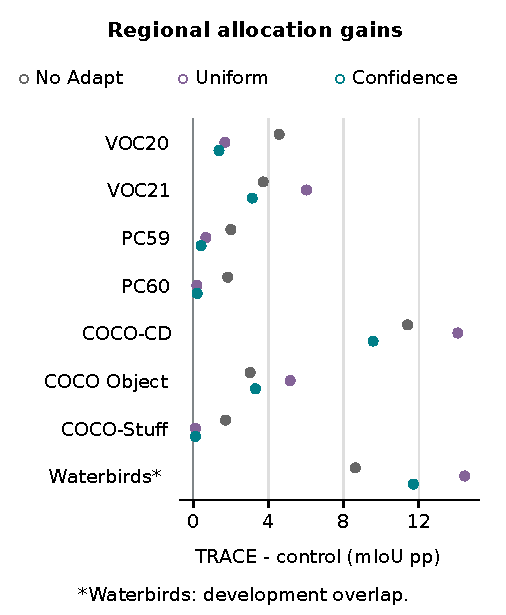
\includegraphics[width=\columnwidth]{figure/tuned/image_full_allocation.pdf}
\caption{TRACE gains over No Adapt and the two matched weighting controls, in mIoU percentage points. Candidates and optimization settings are shared among adapting controls within each dataset. Waterbirds uses the development-overlap protocol described in the setup.}
\label{fig:allocation}
\end{figure}

\begin{figure*}[!t]
\centering
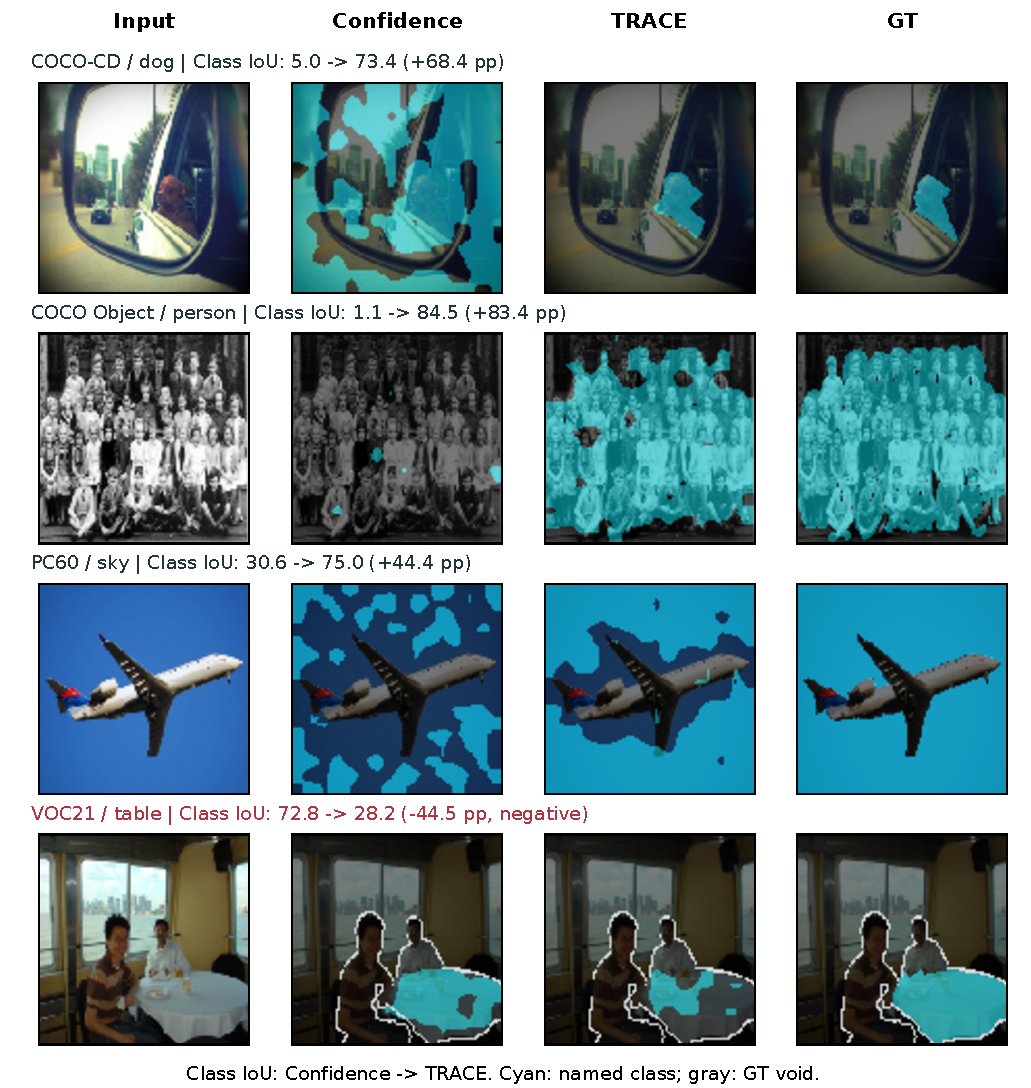
\includegraphics[width=\textwidth]{figure/tuned/image_full_segmentation.pdf}
\caption{Segmentation changes under context-probed regional weighting. Columns show input, matched Confidence allocation, TRACE, and ground truth. Annotations report the displayed image's IoU for the named class. Selected cases include improvements and regressions; identities and selection rules are given in Appendix~\ref{app:figures}.}
\label{fig:segmentation-cases}
\end{figure*}

\subsection{Segmentation Performance in Context}
Published and local references place these allocation gains in the broader OVSS-TTA setting. Table~\ref{tab:tuned-full-reference} lists the clean NACLIP results reported by MLMP~\cite{noori2025mlmp} alongside TRACE. TRACE reaches 53.38 mIoU on VOC21, 30.78 on PC60, 32.67 on COCO Object, and 21.91 on COCO-Stuff, respectively 2.60, 2.79, 3.83, and 0.66 points above the reported MLMP values. VOC20 is close at 83.61 versus 83.76. Because published methods retain their checkpoint, readout, geometry, and optimization protocols, these differences locate reference performance levels; the matched controls in Section~\ref{sec:allocation} isolate the effect of regional weighting under the selected TRACE settings.

\begin{table*}[t]
\caption{Published references (R) and local TRACE (L), mIoU (\%). Reported means and standard deviations follow Table~5, Original NACLIP, of \citet{noori2025mlmp}; No Adapt has no reported dispersion. Local results use seed 0 and TRACE-selected configurations on development-exposed populations. Published and local methods retain their respective protocols.}
\label{tab:tuned-full-reference}
\centering\small
\begin{tabular}{@{}lrrrrr@{}}
\toprule
Method & VOC20 & VOC21 & PC60 & Object & Stuff \\
\midrule
No Adapt (R) & $75.91$ & $45.12$ & $24.95$ & $23.80$ & $18.34$ \\
TENT (R) & $77.00 \pm 0.04$ & $45.65 \pm 0.02$ & $25.29 \pm 0.01$ & $24.88 \pm 0.01$ & $18.76 \pm 0.01$ \\
TPT (R) & $75.93 \pm 0.01$ & $45.17 \pm 0.01$ & $24.98 \pm 0.01$ & $23.84 \pm 0.01$ & $18.35 \pm 0.01$ \\
WATT (R) & $57.73 \pm 0.06$ & $28.58 \pm 0.05$ & $14.77 \pm 0.03$ & $14.14 \pm 0.06$ & $9.49 \pm 0.02$ \\
CLIPArTT (R) & $72.77 \pm 0.14$ & $39.50 \pm 0.04$ & $21.88 \pm 0.03$ & $21.34 \pm 0.03$ & $15.48 \pm 0.01$ \\
MLMP (R) & $83.76 \pm 0.00$ & $50.78 \pm 0.02$ & $27.99 \pm 0.03$ & $28.84 \pm 0.01$ & $21.25 \pm 0.01$ \\
\midrule
TRACE (L) & 83.61 & 53.38 & 30.78 & 32.67 & 21.91 \\
\bottomrule
\end{tabular}
\end{table*}
\begin{table*}[t]
\caption{COCO-CD mIoU (\%) alongside existing local native baselines. TENT is the strongest historical local baseline (72.20). Historical baselines and tuned TRACE retain their respective backends, prompts, and optimization settings; the historical No Adapt uses its native readout.}
\label{tab:tuned-full-cd-reference}
\centering\small
\begin{tabular}{@{}lr@{}}
\toprule
Method / protocol & COCO-CD \\
\midrule
No Adapt (L, historical native) & 61.14 \\
TENT (L, historical native) & 72.20 \\
TPT (L, historical native) & 64.27 \\
MLMP (L, historical native) & 71.01 \\
\midrule
TRACE (L, tuned) & 74.23 \\
\bottomrule
\end{tabular}
\end{table*}


For COCO-CD, which is absent from the published table, local reference runs give 72.20 mIoU for the strongest baseline, TENT, and 74.23 for TRACE. The 2.03-point difference complements the larger matched allocation gain on this dataset. The local reference methods share the ordered image set but retain their method-specific backends and settings (Appendix~\ref{app:native}). PC59 and Waterbirds are reported through the matched controls; no unverified external baseline value is substituted for these protocols.

\subsection{How Much Probing Is Needed?}
A useful diagnostic should add information without requiring several transformed views for every candidate. We compare the context probe ($C$) with a candidate-preserving grayscale-blur probe ($T$) and a two-probe minimum on fixed training-source panels. Uniform and Confidence provide zero-probe controls; an episode-normalized minimum additionally examines the normalization choice. These probe-selection comparisons precede per-dataset tuning and retain their original fixed configurations, separating mode selection from the eight tuned full evaluations.

We choose a common probe rather than a different transformation for each dataset. A fixed calibration rule maximizes the worst-dataset margin over Confidence on PC60 and COCO Object, using measured cost to resolve close choices. It selects $C$ before evaluation on the 256-image panels. Appendix~\ref{app:selection} gives the rule and all calibration outcomes, including the $-0.27$-point PC60 margin.

One context probe retains an advantage over Confidence under all three input orderings: +0.07--0.18 mIoU on PC60 and +2.10--2.92 on COCO Object. The alternatives reveal a tradeoff rather than a universally best probe: $T$ scores higher on Object, while the episode-normalized minimum scores higher on PC60. Collecting a second response is therefore not necessary to improve on confidence weighting, although it can change which dataset benefits most. These order comparisons reuse the same images and assess sensitivity to episode composition, not independent-sample uncertainty.

\subsection{Accuracy--Computation Tradeoff}
One context probe requires $N_{\mathrm{cand}}$ diagnostic inputs, versus $2N_{\mathrm{cand}}$ for a dual-probe minimum. With $P$ input crops and $S$ update steps, a nonempty episode uses
\begin{equation}
N_{\mathrm{enc\ inputs}}=N_{\mathrm{cand}}+(S+2)P,
\end{equation}
including initial readout, adaptation, and final inference. Zero-probe controls omit the first term. Diagnostic \emph{calls} depend on the view batch size; input count is not a wall-time speedup.

The cost is most informative when considered together with the allocation gain. On COCO-CD, TRACE uses 30.56 ms/image versus 23.98 for Confidence and gains 9.57 mIoU; on COCO Object, it uses 320.36 versus 261.11 ms/image and gains 3.31. PC60 uses 84.43 versus 51.90 ms/image for a 0.21-point difference, while COCO-Stuff uses 159.09 versus 101.68 for 0.11 points. These pairs show why a diagnostic should be assessed through both the information it adds and the task's response to it. Appendix~\ref{app:cost} reports costs for every dataset.

Timing covers synchronized model-side execution, including diagnosis, adaptation, reconstruction, and CPU prediction transfer. Data preparation, disk writes, and offline scoring are excluded, and only the first episode is omitted as warmup. These measurements quantify the added diagnostic cost rather than end-to-end data throughput; complete accounting is given in Appendix~\ref{app:cost}.

\subsection{Qualitative Allocation Effects}
Changing regional weights can change the final segmentation even when the initial candidates are identical. Figure~\ref{fig:segmentation-cases} compares Confidence and TRACE on selected images from the full evaluation. The examples make the spatial consequences of the joint update visible and include both improvements and regressions. They illustrate how allocation affects the output; the complete-split measurements above establish its aggregate effect.

\section{Discussion}
The results distinguish confidence in a prediction from information useful for allocating adaptation. TRACE keeps the dense predictor and its candidate set fixed, yet changing the weighting signal yields sizeable improvements on COCO-CD and COCO Object. Context is therefore useful in two distinct ways: it contributes to recognition in the original image, while a controlled change to it supplies an additional observation for selecting self-supervision. This perspective allows adaptation to examine contextual support without discarding context from the final prediction.

TRACE's score expresses relative priority among an image's candidates, not an absolute guarantee that updating on a region is safe. Its normalization removes a common scale factor, including a singleton candidate's positive score; a high score can also preserve a shared prediction error. Connected candidates and confidence top-$K$ determine the granularity and coverage of the decision. The current evidence concerns one backbone and one fixed context transform under the evaluation setting described above. These properties motivate future work on finer within-region allocation and broader diagnostic transformations, while the present study isolates the benefit and cost of the single-probe signal.

\section{Conclusion}
TRACE uses a candidate-preserving context probe to decide how predicted regions share test-time self-supervision. Within-image normalization turns the measured support into relative weights for regional entropy, while adaptation and inference retain the original image. Matched comparisons demonstrate gains beyond initial-confidence weighting, most clearly on COCO-CD and COCO Object. The resulting perspective is to use contextual support not just for recognition, but also to decide which predictions should guide adaptation.

\section*{AI Assistance}
AI assistance was used for source drafting, experimental orchestration, mathematical consistency checks, visualizations, and table-provenance tooling. The authors remain responsible for verifying the experimental evidence and final text.

\bibliography{references}
\clearpage
\appendix
\section{Implementation and Reproduction Protocol}
\label{app:protocol}
\subsection{Method Identity and Execution}
The evaluated method is \texttt{ImageBalancedTRACE} with the single global mode \texttt{C}. It measures one candidate-preserving context-perturbed response, normalizes detached region weights within each source image, and averages the resulting objectives over active source images. The implementation is \path{trace_ovss/method/image_balanced.py}; the full-split worker is \path{tools/evolution_tuning/worker.py}, using the same model, candidate, optimization, and reconstruction code. There is no second probe in the selected mode, semantic-role branch, candidate deletion, dominance attenuation, fragment guard, or CLS loss.

An episode starts from the pretrained parameters and a reset optimizer. The reset model constructs candidates and measures their supports once without gradients. Adaptation reuses fixed candidate locations and weights on unmodified crops, followed by final inference on those crops. Only visual LayerNorm affine parameters change. The four full-split settings execute independently from the same initial model and RNG state; their execution order rotates by episode. Uniform and Confidence use the source-image-normalized objective with weights one and initial confidence, respectively, and compute no diagnostic views. No Adapt performs reset-model inference without candidate diagnosis or optimization.

The runtime uses deterministic PyTorch algorithms with errors on nondeterministic operations, \texttt{CUBLAS\_WORKSPACE\_CONFIG=:4096:8}, deterministic cuDNN, and disabled cuDNN benchmarking. Default attention dispatch remains enabled. Model seed 0 and the original complete evaluation order are fixed. Deterministic execution is not an independent replication or an uncertainty estimate.

\subsection{Images, Crops, Tokens, and Candidates}
A source image is the unit of objective normalization; a crop is an encoder input; a token is a spatial encoder output. The general loader extracts complete sliding-window crops of size $224\times224$ with stride 112, using row-major grid positions and no cross-crop component stitching. Crops retain their source-image IDs. The evaluated configuration first bilinearly resizes every RGB image to $224\times224$, so it yields one crop per source image. This one-crop setting is an evaluation configuration, not the definition of the multi-crop algorithm. ViT-L/14 uses $14\times14$-pixel patches, giving a $16\times16$ spatial-token grid for each crop; 14 is not the crop size.

Let $\mathcal C$ be the supplied text-query vocabulary, including enabled query extensions, and let $\mathcal Y$ be the evaluation-category set. These sets need not coincide. On crop $b$, the reset-model distribution is
\begin{equation}
\pi^0_{b,i}(c\mid x_b)=
\operatorname{softmax}_{c\in\mathcal C}
z^{\mathrm{eval}}_{\theta_0}(x_b)_{i,c}.
\end{equation}
Four-connected components of its token-wise query argmax define proposals $R=(b_R,\Omega_R,c_R)$, with crop index $b_R$, nonempty token set $\Omega_R$, and predicted query $c_R$. Let $j(b)$ map a crop to its source image, and write $j_R=j(b_R)$ for bookkeeping; this is not an additional candidate component. The initial confidence is
\begin{equation}
\kappa_R=\frac{1}{|\Omega_R|}\sum_{i\in\Omega_R}
\pi^0_{b_R,i}(c_R\mid x_{b_R}).
\end{equation}
Proposals from all crops of source image $j$ compete for its first $K$ positions, forming the selected set $\mathcal R_j$. Ranking uses descending $\kappa_R$, descending token area, ascending query index, and ascending component index; stable crop/component enumeration resolves remaining exact ties. There is no overlap union, cross-crop stitching, or minimum-area filter beyond nonemptiness. A valid-token mask excludes geometric padding, not ground-truth background. Distinct query extensions remain distinct components even if they map to the same category.

\subsection{Exact Context Transform and Support}
The C probe changes only the complement of a candidate's input-space mask. Denormalize crop $x_b$ to RGB pixels $u_b\in[0,255]^{3\times224\times224}$ using mean $(122.7709,116.7460,104.0937)$ and standard deviation $(68.5005,66.6322,70.3232)$. For channel $k$, let $\mu_{b,k}$ be its mean over the \emph{entire crop}, including candidate pixels. Define
\begin{align}
A(u_b)&=\operatorname{clip}_{[0,255]}
\left(\operatorname{Shift}\bigl(\mu_b+0.35(u_b-\mu_b)\bigr)\right),\\
\operatorname{Shift}(r,g,b)&=(g,b,r),\\
u_R^{\mathrm{ctx}}&=M_R\odot u_{b_R}
 +(1-M_R)\odot A(u_{b_R}),
\end{align}
where $M_R$ is nearest-neighbor upsampling of the original binary token mask. The view is renormalized before encoding. There is no random transform sampling or learned transform parameter.

The detached C weight is the mean probability of the original query at its original token locations:
\begin{equation}
\rho_R=\frac{1}{|\Omega_R|}
\sum_{i\in\Omega_R}\pi^0_{b_R,i}
\bigl(c_R\mid\operatorname{Norm}(u_R^{\mathrm{ctx}})\bigr).
\label{eq:app-C}
\end{equation}
The diagnostic branch returns token-grid logits without pixel interpolation. It does not re-extract components, match transformed masks, use a probability ratio, or measure a CLS response. Each selected candidate schedules exactly one diagnostic input; view batching changes calls, not that input count. The selected C branch never constructs the unused T view.

Candidate preservation is geometric, not causal isolation. Candidate pixels remain unchanged, but the full-crop channel means depend on them, and the encoder's contextual interactions can mix information inside and outside the mask. The code's compatibility name \texttt{counterfactual\_support} denotes this specified perturbed response, not an identified causal counterfactual or a calibrated probability of update correctness.

\subsection{Dense Readouts and Prompt Entropy}
\label{app:readout}
Diagnosis and final inference use entropy-weighted visual-layer aggregation and normalized mean prompt embeddings. Optimization instead uses uniform mean-layer aggregation and separate prompt embeddings. Both readouts use the last 18 visual outputs of reduced NACLIP ViT-L/14, blocks 7--24 indexed from one, with neighborhood standard deviation 5~\cite{hajimiri2025naclip}. The selected tensors are attention-branch outputs; the ordinary residual and MLP path propagates between blocks.

Let $h_{\ell,b,i}$ be the selected pre-projection output, $\psi_\theta(h)=\mathrm{LN}_{\mathrm{post},\theta}(h)W_{\mathrm{proj}}$, and a hat denote unit-length normalization. For prompt $a\in\{1,\ldots,J\}$ and query $c$, $t_{a,c}$ is the normalized frozen text embedding, and $\bar t_c=\widehat{J^{-1}\sum_at_{a,c}}$, with $J=7$. The multiplier $\lambda=\exp(\ell_{\mathrm{CLIP}})$ is the frozen pretrained logit scale, not a tuned diagnostic temperature. Using $H(p)=-\sum_cp(c)\log p(c)$, inference first computes per-layer query logits and crop-specific entropy weights:
\begin{align}
d_{\ell,b,i}(c)&=\lambda\left\langle
\widehat{\psi_\theta(h_{\ell,b,i})},\bar t_c\right\rangle,\\
v_{\ell,b}&=\frac1N\sum_iH\!\left(
\operatorname{softmax}_c d_{\ell,b,i}\right),\\
w_{\ell,b}&=\frac{\exp(-v_{\ell,b})}{\sum_m\exp(-v_{m,b})}.
\end{align}
Here $N=256$ spatial tokens and the CLS token is excluded. Raw layer outputs are then combined before post-normalization and projection:
\begin{equation}
z^{\mathrm{eval}}_{b,i}(c)=\lambda\left\langle
\widehat{\psi_\theta\!\left(\sum_\ell w_{\ell,b}h_{\ell,b,i}\right)},
\bar t_c\right\rangle.
\end{equation}
This is not an average of per-layer probabilities. Diagnosis uses $\theta_0$; final inference uses the adapted parameters. For optimization, $p^a_{\theta,b,i}=\operatorname{softmax}_c z^{a,\mathrm{adapt}}_{b,i}$, with gradient-bearing prompt-specific logits
\begin{equation}
z^{a,\mathrm{adapt}}_{b,i}(c)=\lambda\left\langle
\widehat{\psi_\theta\!\left(\frac1{18}\sum_\ell h_{\ell,b,i}\right)},
t_{a,c}\right\rangle.
\end{equation}
Thus diagnostic probabilities and adaptation probabilities are related readouts, not interchangeable tensors.

The seven fixed templates are:
\begin{quote}\small
\texttt{itap of a \{\}}\\
\texttt{a bad photo of the \{\}.}\\
\texttt{a origami \{\}.}\\
\texttt{a photo of the large \{\}.}\\
\texttt{a \{\} in a video game.}\\
\texttt{art of the \{\}.}\\
\texttt{a photo of the small \{\}.}
\end{quote}
Prompts and text parameters are frozen. The official OpenAI CLIP \texttt{ViT-L-14.pt} checkpoint~\cite{radford2021clip} has SHA-256 given by concatenating
\begin{quote}\small\ttfamily
b8cca3fd41ae0c99ba7e8951adf17d26\\
7cdb84cd88be6f7c2e0eca1737a03836
\end{quote}
Resource hashes and the exact executed parameter names are retained with the frozen protocols.

\subsection{Source-Image-Normalized Optimization}
Let $\mathcal R_j^+=\{R\in\mathcal R_j:|\Omega_R|>0,\ \rho_R>\epsilon\}$, with $\epsilon=10^{-8}$, and $\mathcal I_+=\{j:\mathcal R_j^+\ne\varnothing\}$. The region entropy and objective are
\begin{align}
\overline H_R(\theta)&=\frac{1}{J|\Omega_R|}
 \sum_{a=1}^J\sum_{i\in\Omega_R}H(p^a_{\theta,b_R,i}),\\
Z_j&=\sum_{Q\in\mathcal R_j^+}\sg(\rho_Q),\\
\alpha_{R\mid j}&=\frac{\sg(\rho_R)}{Z_j},\qquad R\in\mathcal R_j^+,\\
\mathcal L_{\mathrm{TRACE}}(\theta)
 &=\frac1{|\mathcal I_+|}\sum_{j\in\mathcal I_+}
 \sum_{R\in\mathcal R_j^+}\alpha_{R\mid j}\,\overline H_R(\theta).
\label{eq:app-image-loss}
\end{align}
The stop-gradient operator $\sg$ emphasizes that neither supports nor their normalizers are differentiated. Candidate indices, source IDs, and weights remain fixed throughout the episode. Entropy is averaged over prompts and tokens \emph{within each region}, not pooled over all candidate pixels. The original query defines the support measurement but is not a cross-entropy pseudo-label.

Only images with an active nonempty region enter the outer denominator. With none, the tensor helper returns the graph-connected zero $0\sum H$ and the engine skips adaptation. The implementation groups terms by source ID, converts detached scalar weights to the entropy dtype, and uses a double-precision comparison of each summed denominator against $\epsilon$, falling back to one when the denominator does not exceed it. Equation~\ref{eq:app-image-loss} describes the finite active-score case. Crops of one image must share their source ID; treating each crop as a separate image would implement a different objective.

Adam uses $\beta_1=0.9$, $\beta_2=0.999$, and zero weight decay. Trainable parameters include visual input/output LayerNorms and the normalization layers along the executed visual blocks. The final selected block's unused MLP normalization is frozen in the reduced architecture; earlier executed blocks remain differentiable even when their outputs are not selected for readout. Text encoding, projection weights, and the remaining backbone parameters stay frozen. No global image-level or CLS-token objective is added.

\begin{table*}[t]
\caption{TRACE-selected configurations: episode size $B$, learning rate, update steps, and maximum regions per image $K$. Uniform and Confidence reuse these settings without separate tuning. Selection uses 256 calibration images per dataset; the Waterbirds calibration sources overlap its full development population. Historical development exposure is retained.}
\label{tab:tuned-full-configurations}
\centering\small
\begin{tabular}{@{}lrrrr@{}}
\toprule
Dataset & $B$ & Learning rate & Steps & $K$ \\
\midrule
VOC20 & 2 & 0.0015 & 9 & 8 \\
VOC21 & 18 & 0.00125 & 31 & 46 \\
PC59 & 6 & 0.002 & 10 & 46 \\
PC60 & 13 & 0.00375 & 7 & 20 \\
Object & 13 & 0.00375 & 30 & 35 \\
Stuff & 7 & 0.00425 & 10 & 33 \\
COCO-CD & 26 & 0.015 & 5 & 4 \\
Waterbirds & 12 & 0.005 & 4 & 7 \\
\bottomrule
\end{tabular}
\end{table*}


Table~\ref{tab:tuned-full-configurations} specifies the calibration-selected settings. Uniform, Confidence, and TRACE retain the same batch size, learning rate, steps, candidate limit, view batch size, and query-extension flag within each dataset. Only TRACE's settings are searched; the matched controls reuse them, so the comparison tests the effect of replacing its weighting signal at that operating point. Configurations and budgets need not match across datasets or external methods.

\subsection{Pixel Reconstruction and Category Evaluation}
Final reconstruction operates on query logits before category collapsing. For each crop, bilinearly upsample its adapted $16\times16$ query-logit grid to $224\times224$ with \texttt{align\_corners=False}. Place the crop logits at their sliding-window offsets, sum overlaps, and divide by the pixelwise coverage count (clamped below by one). The general implementation uses complete windows, does not add a forced terminal crop, and leaves uncovered positions at zero logits; the present one-crop square configuration covers every evaluated pixel. Crops from one source are reconstructed together, not scored as independent images.

After reconstruction, apply the pixelwise query softmax to obtain $s_c(u)$. If $e(c)$ maps an extension query to its evaluation category, prediction is
\begin{equation}
g_y(u)=\max_{c:e(c)=y}s_c(u),\qquad
\widehat Y(u)=\arg\max_{y\in\mathcal Y}g_y(u).
\end{equation}
This is a maximum after pixel softmax, not a sum of extension probabilities, a category softmax before reconstruction, or a category collapse before candidate construction. Without extensions, $e$ is the identity. Vocabulary files under \path{trace_ovss/resources/class_names/} define categories by nonempty lines and comma-separated extensions within a line: \texttt{cls\_voc20.txt}, \texttt{cls\_voc21.txt}, \texttt{cls\_context59.txt}, \texttt{cls\_context60.txt}, \texttt{cls\_coco\_object.txt}, \texttt{coco\_cd.txt}, \texttt{cls\_coco\_stuff.txt}, and \texttt{waterbirds\_seg.txt}.

The complete evaluation populations are 1,449 images each for VOC20/VOC21, 5,105 each for PC59/PC60, 5,000 each for COCO Object/Stuff, 500 for COCO-CD, and 5,322 for Waterbirds-Seg. The VOC and PC pairs respectively use different category protocols on shared images. Labels are nearest-neighbor resized to the $224\times224$ evaluation grid. The category counts with positive union are 20, 21, 59, 60, 81, 171, 3, and 3 in the order VOC20, VOC21, PC59, PC60, Object, Stuff, CD, and Waterbirds. VOC21, PC60, Object, CD, and Waterbirds include background; VOC20/PC59 exclude background and Stuff uses 171 object/stuff categories. Ignore label 255 is excluded. Pooling intersections $I_y$ and unions $U_y$ over the complete split gives
\begin{equation}
\operatorname{mIoU}=\frac{100}{|\mathcal Y_+|}
\sum_{y\in\mathcal Y_+}\frac{I_y}{U_y},
\qquad \mathcal Y_+=\{y:U_y>0\}.
\end{equation}
This is not an average of per-image or candidate IoUs.

\subsection{Frozen Evidence and Label Separation}
The full evaluation is \path{trace_single_probe_waterbirds_full_20261029_0817} under \path{/home/wwww/hzl/results/}. It imports seven completed calibration selections from \path{trace_single_probe_tuning_20261029_0748}, then selects Waterbirds settings with the same search rule. Eight four-image RGB-only gates across the two stages compare the worker with direct \texttt{ImageBalancedTRACE(view\_mode="C")}; these check implementation identity, not segmentation accuracy. The runtime snapshots, checkpoint, inputs, and selected configurations are bound by their prepared manifests.

All eight complete four-setting prediction sets are sealed before full-evaluation scoring. Prediction processes open RGB inputs but never annotation contents. Separate CPU scoring pools the saved final predictions. Per-dataset prediction/scoring records and the global barrier bind the 32 outcomes. The full continuation's prepared identity is the concatenation
\begin{quote}\small\ttfamily
4f3e54226f99230af48b2105372300d0\\
6f31651515324b3ab99dbe138ff3cfa3
\end{quote}
The fixed C objective and transform are unchanged by parameter search. Saved source snapshots and selected configurations define each full result.

These datasets and inherited starting settings have historical development exposure, including earlier validation-informed choices. New training-source parameter selection does not erase that history. Waterbirds additionally uses 256 existing training examples that also belong to its unchanged 5,322-image evaluation population. Its manifests, selection, and full table explicitly mark \texttt{development\_overlap} with overlap count 256. Thus, prediction-before-scoring separation prevents label access during adaptation, but does not make these experiments untouched held-out evaluations.

\subsection{Per-Dataset Parameter Selection}
For each dataset, a fixed 256-image training-source panel is selected with seed 2027. The C probe, transform, backbone, prompts, readouts, image geometry, and selected visual layers are fixed. Search varies only batch size, learning rate, update steps, and $K$, with at most 80 unique configurations per dataset. Coordinate search proceeds through those four quantities with coarse then local fine candidates; inherited configurations remain eligible. All completed, ineligible, positive, and negative outcomes are retained.

Batch size tests integers 1--16 and its inherited setting, followed by local integer neighbors within three, bounded by 1--32. Learning-rate coarse choices are $10^{-5},3\times10^{-5},10^{-4},3\times10^{-4},5\times10^{-4},0.001,0.002,0.003,0.005,0.008,0.01,0.015,0.02$ plus the inherited value; fine candidates multiply the selected rate by $0.5,0.75,1,1.25,1.5,2$ within $[10^{-6},0.04]$. Steps test $1,3,5,8,12,16,24,32,48$ plus the inherited value, then neighbors within two, bounded by 1--64. $K$ tests $1,2,4,8,16,24,32,48$ plus the inherited value, then neighbors within two, bounded by 1--64. Duplicate configurations are evaluated once.

Selection maximizes pooled calibration mIoU; configurations within 0.02 percentage points of the best prefer lower measured model-side time, then a fixed configuration tuple. Calibration predictions are sealed before each trial score. The seven-dataset stage evaluates 401 configurations; Waterbirds evaluates 54, for 455 in total. All eight selections are fixed before any new full scoring. No full score triggers further search, and Uniform/Confidence are not independently tuned. Historical exposure and Waterbirds overlap remain as stated above.

\section{Objective Algebra and Interpretation}
\label{app:theory}
\subsection{Equal Source Budgets}
Source-image normalization fixes each active image's total objective-coefficient mass. For a finite fixed active set, the within-image weights satisfy
\begin{equation}
\sum_{R\in\mathcal R_j^+}\alpha_{R\mid j}=1,\qquad
\sum_{R\in\mathcal R_j^+}\frac{\alpha_{R\mid j}}{|\mathcal I_+|}
=\frac1{|\mathcal I_+|}.
\end{equation}
In contrast, episode normalization assigns source image $j$ the mass $Z_j/\sum_{k\in\mathcal I_+}Z_k$. Equal image budgets therefore remove this explicit competition through a shared sum-of-support denominator. They do not equalize candidate counts, region areas, gradient norms, Adam updates, or segmentation accuracy. Relative weights and the number of selected regions still affect allocation within an image.

\subsection{Rescaling and Singleton Limits}
Within-image positive rescaling cancels only while the active set and numerical behavior remain unchanged. Replacing every $\rho_R$ in source image $j$ by $\gamma_j\rho_R$, $\gamma_j>0$, leaves $\alpha_{R\mid j}$ and the objective unchanged under those conditions. If an image has exactly one active region, its within-image weight is one and its full objective coefficient is $1/|\mathcal I_+|$, regardless of that region's positive support; other images can still have multiple active regions. With a single active source image, the objective equals the episode-normalized objective for the same candidates and weights. These identities concern normalization, not empirical equivalence between a single probe and two probes.

A low absolute support does not by itself suppress an active image's normalized contribution. Threshold crossings change the active set, and changing the number of active images changes the outer factor. Thus the C score supplies relative allocation within an image, not an absolute rejection or update-safety guarantee.

\subsection{Gradient and Area Boundaries}
Detached coefficients give
\begin{equation}
\nabla_\theta\mathcal L_{\mathrm{TRACE}}
=\frac1{|\mathcal I_+|}\sum_{j\in\mathcal I_+}
\sum_{R\in\mathcal R_j^+}\alpha_{R\mid j}
\nabla_\theta\overline H_R(\theta).
\end{equation}
A token in region $R$ has explicit entropy coefficient
$\alpha_{R\mid j_R}/(|\mathcal I_+|J|\Omega_R|)$.
Region averaging removes a direct area multiplier on the region's total coefficient; it does not remove area-dependent features, candidate selection, or shared-parameter interactions. Across overlapping crops, distinct proposals can also describe overlapping source pixels.

Equal source budgets do not imply batch invariance. Gradients still interact through common visual parameters, and Adam applied to a joint objective is not equivalent to independent per-image updates. Changing episode composition changes those interactions even when all sources retain equal coefficient mass. Neither this algebra nor a high C response establishes that an update improves unknown ground-truth labels.

\section{Global Mode Selection and Training-Source Confirmation}
\label{app:selection}
\subsection{Cohorts and Locked Selection Rule}
One global probe mode is selected using PC60 and COCO Object training-source calibration only. For each dataset, a label-free hash ranking with selection seed 20261029 partitions 128 calibration images and 256 distinct confirmation images, after excluding identifiable historical development IDs and official evaluation identities. Confirmation uses the original sorted order and two permutations with seeds 20261030 and 20261031. Model seed 0 and inherited dataset settings remain unchanged. The three orders reuse the same images and are not independent replicates.

The six arms are episode-normalized minimum (\emph{Old min}), image-normalized Uniform, Confidence, T, C, and minimum. In this comparison, $C_R$ denotes exactly the support $\rho_R$ in Eq.~\ref{eq:app-C}, not an additional score. T measures the original query after replacing context with replicated grayscale followed by $9\times9$ stride-one average blur with padding four and the library's default padded averaging; grayscale weights are $(0.2989,0.5870,0.1140)$. Candidate pixels remain unchanged. Calling that response $T_R$, the minimum alternatives use $\min(T_R,C_R)$. Only Old min uses episode normalization. T and C require one diagnostic input per candidate; either minimum arm requires both. These are fixed alternatives for selection/comparison, not components of the selected C method.

For mode $m\in\{T,C,\min\}$ and calibration dataset $d$, let $\Delta_{d,m}$ be mIoU minus image Confidence. The locked rule maximizes $\min_d\Delta_{d,m}$. Modes within 0.02 percentage points of the best worst-dataset margin are tied; ties prefer fewer actual calibration diagnostic encoder inputs, then larger unweighted mean margin, then the fixed order T, C, minimum. Both datasets and all calibration arms are prediction-sealed before calibration scoring. The selected mode is sealed before any confirmation prediction, and all confirmation arms/orders are sealed before confirmation scoring.

\subsection{Selection Outcome and Scope}
C is selected despite a negative calibration margin on PC60. Its calibration differences from image Confidence are $-0.272957$ pp on PC60 and $+0.579561$ pp on Object; its worst-dataset margin exceeds T's $-0.518667$ and minimum's $-0.308598$. The latter difference is outside the 0.02-pp tie band. Confirmation does not reselect the mode.

\begin{table*}[t]
\caption{Global C was sealed from calibration before confirmation; no reselection. Prospective training-source cohorts under partial documented history only; July candidate pools remain uncertified. Not independent-unseen or full-split evidence. All orders are dependent reorderings, not confidence intervals or significance evidence. Pooled mIoU includes warmup. Calibration128 is separate from confirmation256; all six arms and three confirmation orders are retained.}
\centering\scriptsize
\begin{tabular}{@{}lllrrrrrr@{}}
\toprule
Dataset & Stage & Order & Old min & Image uniform & Image confidence & Image T & Image C & Image min \\
\midrule
PC60 & Calibration & Sorted & 24.846289 & 25.250079 & 25.212533 & 24.693866 & 24.939576 & 24.903935 \\
Object & Calibration & Sorted & 25.799302 & 25.620627 & 25.639792 & 26.711807 & 26.219353 & 25.574809 \\
PC60 & Confirmation & Sorted & 26.569958 & 26.352055 & 26.341809 & 26.287044 & 26.518186 & 26.458232 \\
PC60 & Confirmation & 20261030 & 26.629852 & 26.496603 & 26.386787 & 26.412501 & 26.455814 & 26.456690 \\
PC60 & Confirmation & 20261031 & 26.681803 & 26.358987 & 26.390180 & 26.301490 & 26.544012 & 26.356117 \\
Object & Confirmation & Sorted & 29.955178 & 26.573758 & 27.221342 & 31.100526 & 29.324619 & 29.975437 \\
Object & Confirmation & 20261030 & 30.351900 & 26.833645 & 28.066020 & 30.881844 & 30.166647 & 30.837342 \\
Object & Confirmation & 20261031 & 29.796538 & 26.328251 & 27.041885 & 30.440226 & 29.966576 & 29.832325 \\
\bottomrule
\end{tabular}
\end{table*}
\begin{table*}[t]
\caption{Signed differences versus image confidence in percentage points. Retain negative, zero and positive differences; no post-confirmation mode choice.}
\centering\scriptsize
\begin{tabular}{@{}lllrrrrrr@{}}
\toprule
Dataset & Stage & Order & Old min & Image uniform & Image confidence & Image T & Image C & Image min \\
\midrule
PC60 & Calibration & Sorted & -0.366244 & +0.037546 & +0.000000 & -0.518667 & -0.272957 & -0.308598 \\
Object & Calibration & Sorted & +0.159510 & -0.019165 & +0.000000 & +1.072014 & +0.579561 & -0.064984 \\
PC60 & Confirmation & Sorted & +0.228150 & +0.010246 & +0.000000 & -0.054764 & +0.176377 & +0.116423 \\
PC60 & Confirmation & 20261030 & +0.243065 & +0.109815 & +0.000000 & +0.025714 & +0.069026 & +0.069902 \\
PC60 & Confirmation & 20261031 & +0.291623 & -0.031193 & +0.000000 & -0.088690 & +0.153832 & -0.034063 \\
Object & Confirmation & Sorted & +2.733836 & -0.647584 & +0.000000 & +3.879184 & +2.103277 & +2.754095 \\
Object & Confirmation & 20261030 & +2.285879 & -1.232375 & +0.000000 & +2.815823 & +2.100626 & +2.771322 \\
Object & Confirmation & 20261031 & +2.754653 & -0.713634 & +0.000000 & +3.398341 & +2.924691 & +2.790440 \\
\bottomrule
\end{tabular}
\end{table*}


Selected C exceeds image Confidence in all three confirmation orders on both datasets: $+0.069026$ to $+0.176377$ pp on PC60 and $+2.100626$ to $+2.924691$ pp on Object. This is not best-arm superiority. Old min is higher than C in all three PC60 orders, and T is higher than C in all three Object orders. The tables retain every arm and signed difference, including negative results.

The cohort evidence is prospective only relative to the documented exclusion inventory. Exact membership of historical July 4,096-image candidate pools remains uncertified because surviving loader/train-split records do not establish the necessary mapping. Neither global never-seen status nor exhaustive historical exclusion is established. The cohort source is \path{trace_image_budget_20261029_0233}, including \texttt{SELECTION\_SEALED.json}, under the results directory above. The selection seal is pinned by the new full suite. Neither these dependent reorderings nor the full seed-0 run supplies independent confidence intervals, seed dispersion, bootstrap inference, or significance.

The common C mode is retained during subsequent per-dataset parameter search and all eight full evaluations. The probe-selection tables above retain their own fixed configurations and training-source populations. They are not the tuned full results in main-paper Table~\mainref{tab:tuned-full-comparison}, and do not select a different probe for each dataset.

\section{Computation and Timing Scope}
\label{app:cost}
The selected C method independently constructs candidates, evaluates one context view per selected candidate, adapts, and reconstructs predictions. Uniform and Confidence omit diagnostic forwards but retain candidate construction and optimization. For $P$ input crops, $S$ executed update steps, and $n$ selected candidates in a nonempty episode, the standard encoder-input schedules are $(S+2)P+n$ for C and $(S+2)P$ for its zero-view controls: one initial candidate pass, $S$ adaptation passes, and one final inference pass. T has the same diagnostic-input count as C; a two-view minimum adds $2n$ instead. Actual counters, rather than this nonempty-episode formula, govern empty or skipped episodes.

Diagnostic inputs and batched encoder calls are different costs. A one-probe design halves diagnostic inputs relative to a two-probe design with identical candidates, not total model work or wall time. The full suite contains No Adapt, Uniform, Confidence, and C, but no minimum arm; it therefore provides no full-split two-probe timing comparison. No Adapt uses one reset inference pass and no adaptation. Historical cohort timing ratios are not transferred to the tuned full results.

Full-split costs use synchronized model-side timers around reset, candidate construction, requested diagnostics, adaptation, final reconstruction, and CPU prediction transfer. They include the full worker's observation-only finite-value checks and accounting hooks; these checks abort on nonfinite logits, gradients, parameters, or Adam state without changing the objective, adding encoder passes, or certifying semantic safety. Hook setup and artifact serialization are outside the timer. Model loading, RGB decode, H2D/geometry preparation, disk writes, and offline scoring are excluded. This is not end-to-end throughput. Episode 0 is omitted from timing only; all its predictions, accuracy counts, and encoder work are retained. The timing denominator is therefore total source images minus the first episode, whereas work counts use all source images.

\begin{table*}[t]
\caption{Model-side time per image (ms), excluding the first episode as warmup. Timing includes reset, candidate admission, diagnostic views, optimization, and final readout; it excludes data loading, disk writes, and offline scoring. Extra time is relative to Confidence under the same TRACE-selected configuration.}
\label{tab:tuned-full-cost}
\centering\small
\begin{tabular}{@{}lrrr@{}}
\toprule
Dataset & Confidence (ms) & TRACE (ms) & Extra time \\
\midrule
VOC20 & 153.46 & 165.99 & +8.17\% \\
VOC21 & 273.45 & 343.73 & +25.70\% \\
PC59 & 115.71 & 186.77 & +61.41\% \\
PC60 & 51.90 & 84.43 & +62.68\% \\
Object & 261.11 & 320.36 & +22.69\% \\
Stuff & 101.68 & 159.09 & +56.45\% \\
COCO-CD & 23.98 & 30.56 & +27.45\% \\
Waterbirds & 26.46 & 37.99 & +43.58\% \\
\bottomrule
\end{tabular}
\end{table*}


The calibration/confirmation cost tables below retain all six independently executed arms and every order on their own cohorts. Their timing scope and warmup convention match the definitions above, but they are separate measurements from the guarded full-split worker. They do not establish equal-budget comparisons with external methods.

\begin{table*}[t]
\caption{Global C was sealed from calibration before confirmation; no reselection. Prospective training-source cohorts under partial documented history only; July candidate pools remain uncertified. Not independent-unseen or full-split evidence. All orders are dependent reorderings, not confidence intervals or significance evidence. Synchronized model-side ms/image; $N$ excludes only episode 0. Includes reset, candidates, requested views, adaptation, final inference and CPU prediction transfer. Excludes model loading, RGB decode, H2D/geometry preparation, disk writes and scoring; not end-to-end throughput.}
\centering\scriptsize
\begin{tabular}{@{}lllrrrrrrr@{}}
\toprule
Dataset & Stage & Order & $N$ & Old min & Image uniform & Image confidence & Image T & Image C & Image min \\
\midrule
PC60 & Calibration & Sorted & 119 & 142.189 & 69.796 & 69.663 & 106.605 & 106.839 & 142.796 \\
Object & Calibration & Sorted & 114 & 327.658 & 216.959 & 216.465 & 270.054 & 271.848 & 326.164 \\
PC60 & Confirmation & Sorted & 247 & 136.390 & 66.483 & 66.448 & 101.829 & 102.030 & 136.874 \\
PC60 & Confirmation & 20261030 & 247 & 136.450 & 66.446 & 66.487 & 101.851 & 102.141 & 136.939 \\
PC60 & Confirmation & 20261031 & 247 & 136.319 & 66.588 & 66.424 & 101.655 & 101.789 & 136.771 \\
Object & Confirmation & Sorted & 242 & 314.542 & 209.470 & 209.574 & 261.083 & 264.232 & 316.154 \\
Object & Confirmation & 20261030 & 242 & 314.703 & 209.650 & 209.782 & 261.031 & 264.567 & 315.874 \\
Object & Confirmation & 20261031 & 242 & 315.985 & 210.886 & 210.439 & 261.734 & 265.267 & 317.099 \\
\bottomrule
\end{tabular}
\end{table*}
\begin{table*}[t]
\caption{Actual diagnostic encoder inputs / total encoder inputs per source image. $N$ includes all images including warmup, unlike timing. Calls and all totals are retained in provenance.}
\centering\scriptsize
\begin{tabular}{@{}lllrrrrrrr@{}}
\toprule
Dataset & Stage & Order & $N$ & Old min & Image uniform & Image confidence & Image T & Image C & Image min \\
\midrule
PC60 & Calibration & Sorted & 128 & 43.688 / 56.688 & 0.000 / 13.000 & 0.000 / 13.000 & 21.844 / 34.844 & 21.844 / 34.844 & 43.688 / 56.688 \\
Object & Calibration & Sorted & 128 & 67.609 / 98.609 & 0.000 / 31.000 & 0.000 / 31.000 & 33.805 / 64.805 & 33.805 / 64.805 & 67.609 / 98.609 \\
PC60 & Confirmation & Sorted & 256 & 43.703 / 56.703 & 0.000 / 13.000 & 0.000 / 13.000 & 21.852 / 34.852 & 21.852 / 34.852 & 43.703 / 56.703 \\
PC60 & Confirmation & 20261030 & 256 & 43.703 / 56.703 & 0.000 / 13.000 & 0.000 / 13.000 & 21.852 / 34.852 & 21.852 / 34.852 & 43.703 / 56.703 \\
PC60 & Confirmation & 20261031 & 256 & 43.703 / 56.703 & 0.000 / 13.000 & 0.000 / 13.000 & 21.852 / 34.852 & 21.852 / 34.852 & 43.703 / 56.703 \\
Object & Confirmation & Sorted & 256 & 67.680 / 98.680 & 0.000 / 31.000 & 0.000 / 31.000 & 33.840 / 64.840 & 33.840 / 64.840 & 67.680 / 98.680 \\
Object & Confirmation & 20261030 & 256 & 67.680 / 98.680 & 0.000 / 31.000 & 0.000 / 31.000 & 33.840 / 64.840 & 33.840 / 64.840 & 67.680 / 98.680 \\
Object & Confirmation & 20261031 & 256 & 67.680 / 98.680 & 0.000 / 31.000 & 0.000 / 31.000 & 33.840 / 64.840 & 33.840 / 64.840 & 67.680 / 98.680 \\
\bottomrule
\end{tabular}
\end{table*}


\section{Qualitative Evidence and Selection Limits}
\label{app:figures}
A candidate illustration is an input-space view paired with a stored token-space measurement. The full C artifacts retain candidate query/category identity, source/crop IDs, confidence, measured C, detached objective coefficient, and lossless original token masks. Candidate-preserving context views can be rendered from these masks and source RGB inputs without a new diagnostic inference. Display names denote predicted queries or their recorded category mapping, not ground-truth identification. The original token footprint, not a newly segmented region in the transformed image, defines the displayed support.

Unmeasured T is unavailable in the C full suite, not zero. The independently executed No Adapt setting supplies complete reset-model category predictions; the candidate receipt itself is not such a map. The figures use the saved matched Confidence/C outputs and measured C supports. No old two-view score or segmentation is substituted into these examples.

The teaser selects two support extremes without ground truth. Within the first 400 images of each frozen dataset order, eligible candidates are non-background predictions with $\kappa_R\geq0.9$ and 16--192 native tokens. The highest C response in PC60 and lowest in Object are selected, breaking ties by source-image index then receipt candidate index. Image indices are zero-based; candidate indices refer to the recorded episode receipt. Exact identities and supports are retained in \path{figure/tuned/image_full_provenance.json}. The rendered context views use the float32 transform and original $16\times16$ masks; displayed supports are saved measurements, not new model evaluations.

Segmentation cases are offline named-class IoU extremes among the first 400 images per dataset. For each image, choose its largest non-background ground-truth category with at least 128 valid pixels, breaking area ties by the lowest category ID. Compute that single category's IoU for saved Confidence and C predictions. Select the largest C-minus-Confidence difference for CD, Object, and PC60, and the smallest for VOC21; ties use the lowest image index. These values are per-image named-class IoUs, not image-averaged or dataset mIoU. The Confidence column is the matched allocation control, not MLMP.

Selected extremes illustrate both directions of change, not their frequency. Ground truth enters segmentation-display selection only after the global prediction seal and never enters adaptation or mode selection. Exact identities, selection rules, stored measurements, rendering checks, and source seals are in \path{figure/tuned/image_full_provenance.json}. The displays do not establish a causal effect of an individual region's coefficient under the joint update.

\section{Reported and Local Reference Protocols}
\label{app:native}
Reported operating points (R) and local measurements (L) have different evidential roles. For VOC20, VOC21, PC60, COCO Object, and COCO-Stuff, MLMP's main Table 5 reports clean NACLIP ViT-L/14 values 83.76, 50.78, 27.99, 28.84, and 21.25~\cite{noori2025mlmp}. TRACE scores are 83.614345, 53.380927, 30.782843, 32.671159, and 21.911536. Four exceed the reported values, while VOC20 is lower by 0.145655 pp. A shared backbone family does not certify identical checkpoints, query vocabularies, loaders, readouts, optimization budgets, or tuning histories.

COCO-CD has a separate completed local native reference. The adapting native baselines retain their backend behavior and prompts with learning rate 0.001 and 10 updates, whereas C uses Table~\ref{tab:tuned-full-configurations}. The best retained native baseline is TENT~\cite{wang2021tent} at 72.200299, compared with C at 74.231207. These runs share the ordered image population, but differ in episode composition and native protocols; the 2.030908-pp difference is not an equal-budget attribution. The matched No Adapt in main-paper Table~\mainref{tab:tuned-full-comparison}, rather than the historical native No Adapt, establishes the current method's adaptation gain.

Published statistics remain attributed to their sources and are not pooled with local deterministic results. Existing published MLMP values are used without additional MLMP reruns. No local WATT or CLIPArTT evaluation is claimed. The within-implementation Uniform/Confidence/C controls, training-source selection comparisons, cross-paper operating points, and local native CD reference answer different questions and are not interchangeable.


\end{document}
